\chapter{Programmablaufprotokolle}

Zum Testen wurde folgendes Beispiel ausgewählt:

Nach dem Anmelden drückt man zuerst auf "`Schule"' und dort "`Neue Schule anlegen"'. Die neue Schule hat den Namen Musterschule und befindet sich in der Musterstraße 1 in 01234 Musterstadt. Nach dem Eintragen der Daten kann diese gespeichert werden und die neu angelegte Schule erscheint in der Liste. 

Nun ist es möglich, bei "`Schüler"' neue Schüler hinzuzufügen. Wir nehmen Erika Musterfrau, Max Mustermann und Viktor Vorbeeld. Erika besucht die 9. Klasse, ebenso Max und Viktor. Alle 3 gehen auf die eben angelegte Musterschule und wohnen in der Mustergasse in 01234 Musterstadt. 

Jetzt ist es möglich, über "`Fächer"' ein neues Fach anzulegen, in unserem Beispiel Biologie. 

Nun kann man zu "`Zirkel"' wechseln und einen neuen im Fach Biologie, Klassenstufe 9 anlegen. Dabei muss man beachten, dass man das richtige Schuljahr eingestellt hat.

Klickt man nun auf "`Teilnehmer verwalten"', werden alle Schüler der Klassenstufe 9 angezeigt, also auch unsere drei aus der Mustergasse. Von diesen drei Schülern wollen aber nur Erika und Viktor am Biologiezirkel teilnehmen, deshalb klickt man bei den beiden auf Eintragen. Sie sind jetzt in dem Zirkel und bekommen Aufgaben zugeschickt. Durch Klicken auf den Zirkelnamen kommt man zurück zur Übersichtseite von dem Zirkel, wo alle beide registrierten Teilnehmer aufgeführt sind.

Bei dem Zirkel kann man mittels "`Aufgaben verwalten"' die einzelnen Aufgabenserie mit der jeweils maximal möglichen Punktzahl anlegen. Unser Beispiel enthält 5 Serien mit 17, 18, 20, 19 und 24 erreichbaren Punkten. 

Wenn man in der Übersicht auf eine Aufgabenserie klickt, erscheint eine Seite zum Eintragen der von den Schülern erreichten Punkte. Erika hat jeweils 4,8,2 und 13 Punkte erhalten. die vorletzte Aufgabenserie hatte sie vergessen abzuschicken, dadurch wurden ihr keine Punkte für den einen Brief erteilt. Sie hat insgesamt 27 Punkte, das entspricht 28 \% der Gesamtpunktzahl von 98 Punkten. Viktor war besser und hat 11,8,19 und 17 Punkte bekommen. Auf die erste Aufgabenserie hat er 0 Punkte bekommen, das heißt nicht, dass er nichts abgeschickt hat, sondern er hat einfach keine richtigen Lösungen gehabt. Im Unterschied zu Erika bleibt das Feld bei der Aufgabenserie nicht frei, sondern es stehen 0 Punkte darin. Viktor hat insgesamt 55 Punkte bekommen, also rund 56 \%. Diese Zahlen sind nach jedem Speichern der erreichten Punkte und über "`Auswertung"' beim Zirkel zu sehen.

\begin{figure}[h]
	\centering
	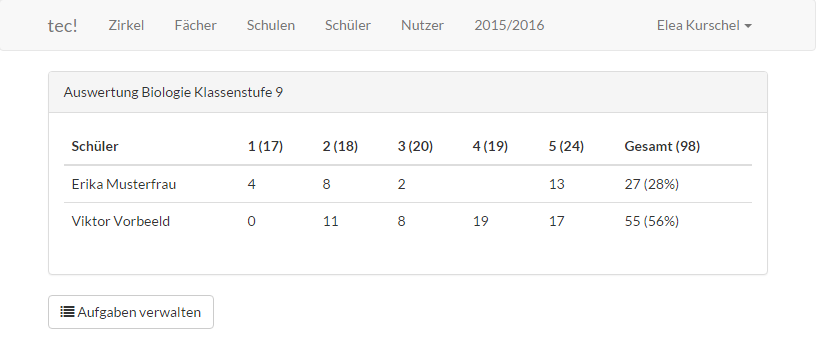
\includegraphics[scale=.50]{bilder/Protokoll_Auswertung.png}
	\caption{Beispiel Auswertung Zirkel}
	%\label{abb:beispiel}
\end{figure}

Außerdem kann man nun unter der Musterschule sehen, welche die aktiven Teilnehmer sind. Es sind nur Erika und Viktor, da sie im Gegensatz zu Max tatsächlich an einer Korrespondenz teilnehmen.

\begin{figure}[h]
	\centering
	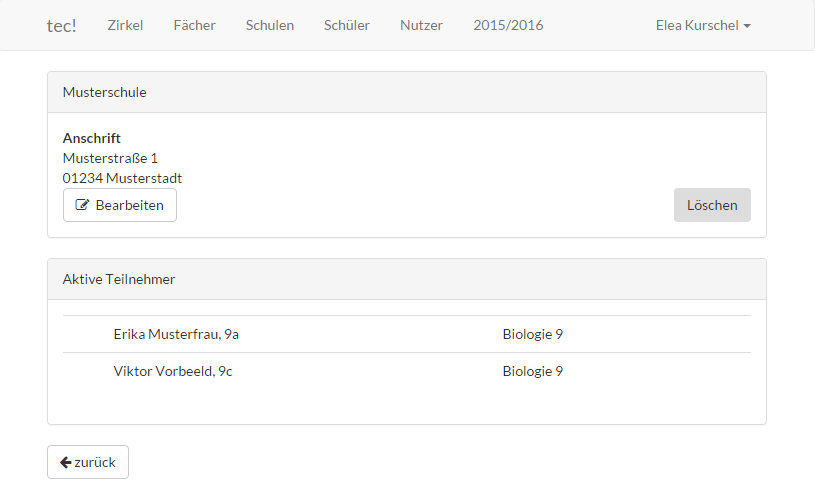
\includegraphics[scale=.50]{bilder/Protokoll_Schule.png}
	\caption{Beispiel Teilnehmer einer Schule}
	%\label{abb:beispiel}
\end{figure}
